% Classes of optimization problems, and the modeling paradigms that cut across
% them.
%
% Re-authored to replace media/classification.png, which was a verbatim SCAN of
% Biegler (2010), Figure 1.1 ("Classes of optimization problems"), caption and
% all -- not searchable, not scalable, not greyscale-checkable, and not ours.
%
% It is an ADAPTATION, not a redrawing. Four things are different, each asked
% for by Prof. Dowling (2026-08-25):
%
%   1. COVERAGE IS COLOUR-CODED. "I want to color-code the problem classes we
%      will not discuss this semester."
%   2. THE CONVEX BRANCH IS A NESTING, NOT A FAN. "Where does conic
%      optimization fit into this diagram?" Biegler's flat Convex -> {LP, QP}
%      cannot express LP < QP < SOCP < SDP, so the four are drawn as a chain
%      of inclusions instead of as siblings.
%   3. THE MIXED-INTEGER BRANCH IS ALSO A NESTING, and MIQP is in it. "What
%      about MIQPs and other specific problem types?" Biegler's chain runs
%      MINLP -> MILP -> IP downward, which reads as specialisation but is drawn
%      as descent; here it runs IP < MILP < MIQP < MINLP so both chains read
%      the same direction (special -> general).
%   4. THERE IS A PARADIGM BAND AT THE BOTTOM. "I also want to have boxes at
%      the bottom that highlight modeling paradigms, such as stochastic
%      programming and dynamic optimization."
%
% ---------------------------------------------------------------------------
% THE PEDAGOGICAL POINT OF THE BAND: the paradigms are ORTHOGONAL to the tree,
% not another branch of it. A stochastic program can be an LP or an MINLP; a
% dynamic optimization problem discretizes INTO an NLP. So the band is drawn
% as a different KIND of object -- rounded tags inside a dashed enclosure, no
% tree edges, one arrow pointing back up at the whole tree rather than at any
% node in it. If it were drawn as more tree nodes it would teach the opposite
% of what it is for. The five entries are the course's own Part I list
% (see ../../optimization-private/lecture-notes/lectures/introduction.tex,
% "The semester").
%
% ---------------------------------------------------------------------------
% GREYSCALE. The colour policy (figures/dowling.mplstyle header, and
% figures/README.md "Course additions") is: a distinction may be carried by
% colour, but NEVER by colour alone. Coverage therefore has THREE redundant
% encodings, two of which are colour-free:
%
%     covered            white fill      SOLID   rule    black text
%     modeled-only       blue tint       DASHED  rule    black text
%     not covered        grey tint       DOTTED  rule    grey text
%
% The two tints are deliberately close in luminance -- they are tints, so they
% must be, to keep the text on them readable. The dash pattern is what a
% photocopy reads. The legend strip repeats all three treatments, so a reader
% in black and white decodes the figure from the legend alone.
%
% ---------------------------------------------------------------------------
% NO \ref/\eqref anywhere: this file is rendered standalone by figures/Makefile
% as well as \input by the handout, and a cross-reference would print "??".

% Okabe-Ito blue at low saturation. The hue is the colour-vision-safe blue from
% the house palette; the tint keeps black text on it readable.
\definecolor{classblue}{HTML}{D6E7F2}
\definecolor{bandgrey}{HTML}{F4F4F4}

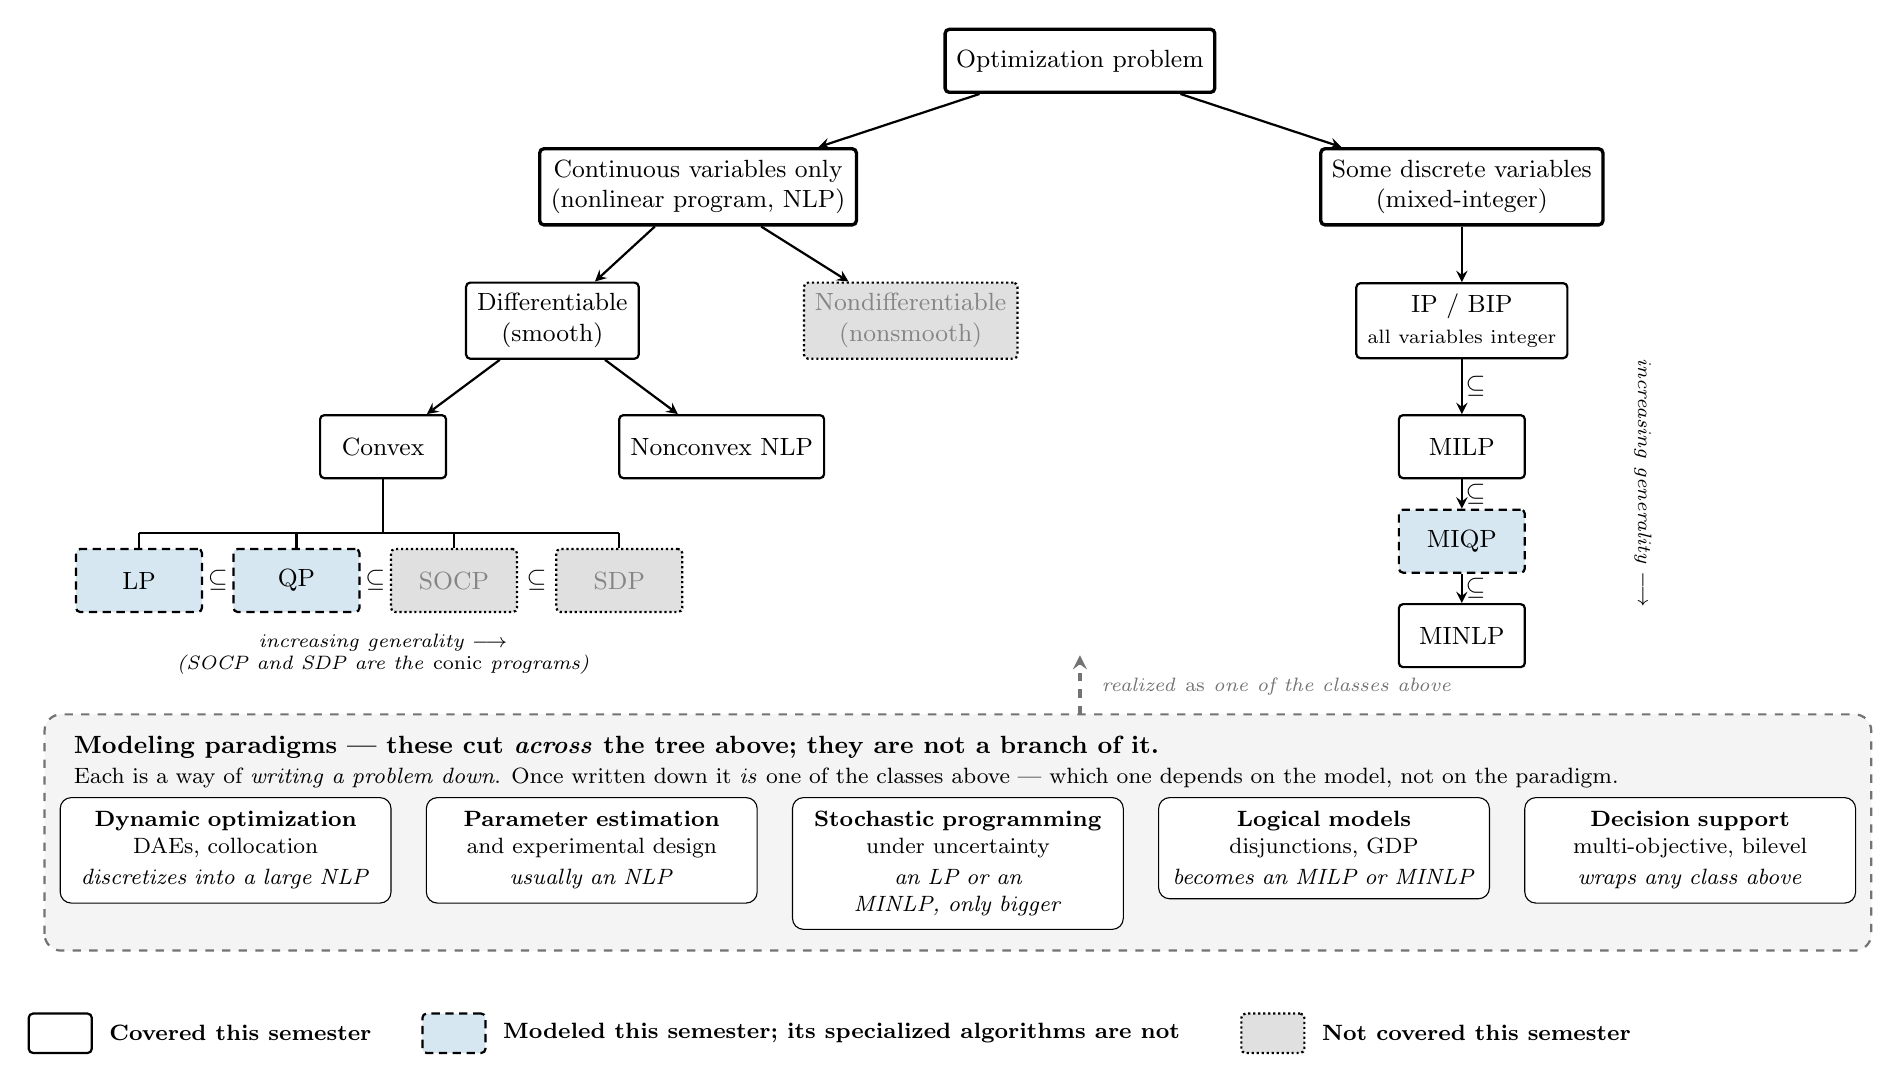
\begin{tikzpicture}[
  every node/.style = {font=\small},
  % --- coverage treatments ------------------------------------------------
  cov/.style     = {draw, thick, rectangle, rounded corners=1.5pt, fill=white,
                    align=center, inner sep=4pt, minimum height=8mm,
                    minimum width=1.6cm},
  modeled/.style = {cov, densely dashed, fill=classblue},
  uncov/.style   = {cov, densely dotted, fill=black!12, text=black!48},
  struct/.style  = {cov, very thick},
  % --- edges ---------------------------------------------------------------
  go/.style      = {->, >=stealth, thick},
  plain/.style   = {thick},
  lbl/.style     = {font=\scriptsize\itshape, align=center, inner sep=2pt},
  sub/.style     = {font=\small, inner sep=1pt},
  % --- the paradigm band ---------------------------------------------------
  % anchor=north so five tags of different heights hang from one line.
  % Hyphenation off: "Stochastic pro-gramming" across two lines is worse than
  % a short line.
  tag/.style     = {draw, rounded corners=4pt, thin, fill=white, anchor=north,
                    align=center, text width=3.85cm, inner sep=5pt,
                    font=\footnotesize, hyphens/.code={},
                    execute at begin node={\hyphenpenalty=10000\exhyphenpenalty=10000}},
]

% =========================================================================
% The paradigm band is drawn FIRST so it sits behind everything. Drawing it
% with an explicit rectangle rather than \usetikzlibrary{fit,backgrounds}
% keeps figures/preamble.tex unchanged.
% =========================================================================
\fill[bandgrey, rounded corners=6pt] (-13.2,-11.30) rectangle (10.0,-8.30);
\draw[dashed, thick, rounded corners=6pt, black!55]
      (-13.2,-11.30) rectangle (10.0,-8.30);

% =========================================================================
% THE TREE
% =========================================================================
\node[struct] (root) at (-0.05,0) {Optimization problem};

\node[struct] (cont) at (-4.9,-1.6)
      {Continuous variables only\\ (nonlinear program, NLP)};
\node[struct] (mip)  at (4.8,-1.6)
      {Some discrete variables\\ (mixed-integer)};

\draw[go] (root) -- (cont);
\draw[go] (root) -- (mip);

% --- continuous branch ---------------------------------------------------
\node[cov]   (smooth)    at (-6.75,-3.3) {Differentiable\\ (smooth)};
\node[uncov] (nonsmooth) at (-2.2,-3.3)  {Nondifferentiable\\ (nonsmooth)};

\draw[go] (cont) -- (smooth);
\draw[go] (cont) -- (nonsmooth);

\node[cov] (convex)    at (-8.9,-4.9) {Convex};
\node[cov] (nonconvex) at (-4.6,-4.9) {Nonconvex NLP};

\draw[go] (smooth) -- (convex);
\draw[go] (smooth) -- (nonconvex);

% The convex classes as a CHAIN OF INCLUSIONS, which is the whole reason this
% figure differs from Biegler's. LP c QP c SOCP c SDP: every linear program is
% a quadratic program with a zero Hessian, every convex QP (indeed every convex
% QCQP) is representable as a second-order cone program, and every SOCP is a
% semidefinite program with block-diagonal structure.
\node[modeled] (lp)   at (-12.0,-6.6) {LP};
\node[modeled] (qp)   at (-10.0,-6.6) {QP};
\node[uncov]   (socp) at (-8.0,-6.6)  {SOCP};
\node[uncov]   (sdp)  at (-5.9,-6.6)  {SDP};

\node[sub] at (-11.0,-6.6) {$\subseteq$};
\node[sub] at (-9.0,-6.6)  {$\subseteq$};
\node[sub] at (-6.95,-6.6) {$\subseteq$};

% comb connector: all four hang off "Convex"
\draw[plain] (convex.south) -- (-8.9,-6.0);
\draw[plain] (-12.0,-6.0) -- (-5.9,-6.0);
\draw[plain] (-12.0,-6.0) -- (lp.north);
\draw[plain] (-10.0,-6.0) -- (qp.north);
\draw[plain] (-8.0,-6.0)  -- (socp.north);
\draw[plain] (-5.9,-6.0)  -- (sdp.north);

\node[lbl, anchor=north] at (-8.9,-7.2) {increasing generality $\longrightarrow$\\
      (SOCP and SDP are the \emph{conic} programs)};

% --- mixed-integer branch ------------------------------------------------
% Same reading direction as the convex chain: special at the top, general at
% the bottom. IP c MILP c MIQP c MINLP.
\node[cov]     (ip)    at (4.8,-3.3) {IP / BIP\\ \scriptsize all variables integer};
\node[cov]     (milp)  at (4.8,-4.9) {MILP};
\node[modeled] (miqp)  at (4.8,-6.1) {MIQP};
\node[cov]     (minlp) at (4.8,-7.3) {MINLP};

\draw[go] (mip)  -- (ip);
\draw[go] (ip)   -- node[sub, right] {$\subseteq$} (milp);
\draw[go] (milp) -- node[sub, right] {$\subseteq$} (miqp);
\draw[go] (miqp) -- node[sub, right] {$\subseteq$} (minlp);

\node[lbl, anchor=west, rotate=-90] at (7.1,-3.7)
      {increasing generality $\longrightarrow$};

% =========================================================================
% THE PARADIGM BAND -- contents
% =========================================================================
\node[anchor=north west, align=left, font=\small] at (-12.95,-8.45)
      {\textbf{Modeling paradigms --- these cut \emph{across} the tree above; they are not a branch of it.}\\
       \footnotesize Each is a way of \emph{writing a problem down}. Once written down it \emph{is} one of the
       classes above --- which one depends on the model, not on the paradigm.};

\node[tag] (par1) at (-10.90,-9.35)
      {\textbf{Dynamic optimization}\\ DAEs, collocation\\[2pt]
       \emph{discretizes into a large NLP}};
\node[tag] (par2) at (-6.25,-9.35)
      {\textbf{Parameter estimation}\\ and experimental design\\[2pt]
       \emph{usually an NLP}};
\node[tag] (par3) at (-1.60,-9.35)
      {\textbf{Stochastic programming}\\ under uncertainty\\[2pt]
       \emph{an LP or an MINLP, only bigger}};
\node[tag] (par4) at (3.05,-9.35)
      {\textbf{Logical models}\\ disjunctions, GDP\\[2pt]
       \emph{becomes an MILP or MINLP}};
\node[tag] (par5) at (7.70,-9.35)
      {\textbf{Decision support}\\ multi-objective, bilevel\\[2pt]
       \emph{wraps any class above}};

% One arrow, pointing at the TREE AS A WHOLE rather than at any node in it.
% That is the orthogonality claim, drawn.
\draw[->, >=stealth, very thick, dashed, black!55] (-0.05,-8.30) -- (-0.05,-7.55);
\node[lbl, anchor=west, black!55] at (0.15,-7.95)
      {realized \emph{as} one of the classes above};

% =========================================================================
% LEGEND -- repeats all three treatments, so a black-and-white reader can
% decode the figure from here without seeing a single hue.
% =========================================================================
\node[cov, minimum width=8mm, minimum height=5mm, inner sep=2pt] at (-13.0,-12.35) {};
\node[anchor=west, font=\footnotesize] at (-12.5,-12.35)
      {\textbf{Covered this semester}};

\node[modeled, minimum width=8mm, minimum height=5mm, inner sep=2pt] at (-8.0,-12.35) {};
\node[anchor=west, font=\footnotesize] at (-7.5,-12.35)
      {\textbf{Modeled this semester; its specialized algorithms are not}};

\node[uncov, minimum width=8mm, minimum height=5mm, inner sep=2pt] at (2.4,-12.35) {};
\node[anchor=west, font=\footnotesize] at (2.9,-12.35)
      {\textbf{Not covered this semester}};

\end{tikzpicture}
